\subsection{Two Degrees of freedom Controller}
\label{2dof}
A Two Degrees of freedom Controller (2-DOF) strategy \cite{kmm07} was
implemented remotely on SBHS through virtual lab. A block diagram for
the same is as shown in the Figure \ref{2doffig}. After performing the
step test, the second order transfer funtion obtained was  
\begin{align*}
G(s)&=\frac {1.029}{(71.16s+1)(s+1)}
\end{align*}
with time constant $\tau_1 = 71.16 sec$, $\tau_2 = 1 sec$  and gain $K=1.029$.
%
\begin{figure}
\centering
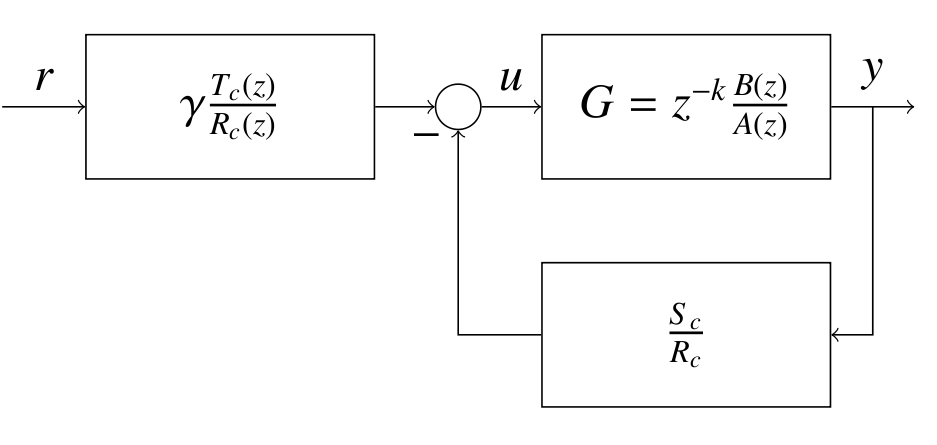
\includegraphics[width=\linewidth]{figures/2dof.png}
\caption{Two Degrees of freedom Controller structure}
\label{2doffig}
\end{figure}
%
For rise time = 20 seconds and Overshoot of 5\%, the various
controller parameters obtained are
\begin{align*}
R_c &=  0.0143941 -  0.0345042z^{-1}  + \\&0.0265766z^{-2} - 0.0064665z^{-3}  \\
S_c &=  0.0045849  - 0.0045528z^{-1}\\
T_c &= 1.  - 0.9929982z^{-1}\\
\gamma &= 0.004589
\end{align*}
The response of the controller implented on SBHS virtually is as shown
in the Figure \ref{2dofresp}.


\begin{figure}
\hspace{-0.2in}
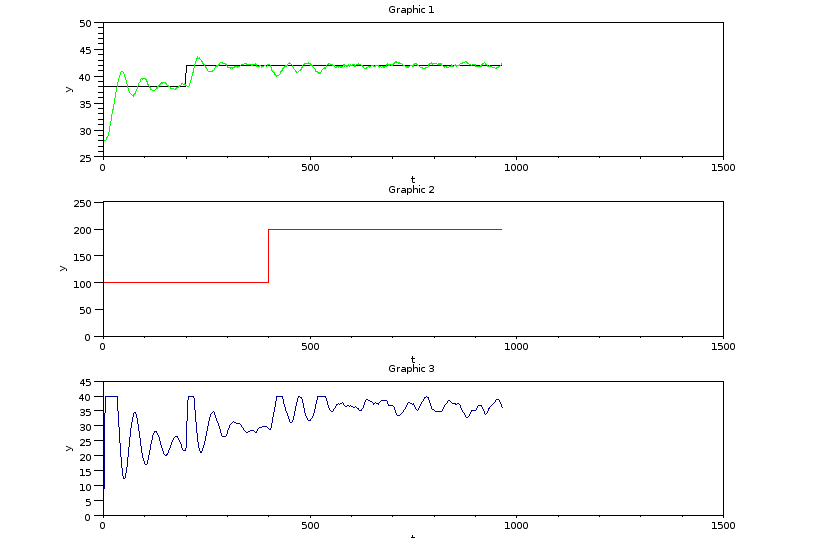
\includegraphics[width=1.2\linewidth]
{figures/twodof_disturbance_intranet.png}
\caption{2-DOF controller implementation: temperature, fan speed,
  heater duty}
\label{2dofresp}
\end{figure}

